\section{Taxonomy}
\label{sec:tax}
We use a taxonomy as the external classification knowledge for
conceptualizing the arguments of verbs.
A taxonomy is a direct acyclic graph $(V, E)$,
Here, $V$ is a set of terms, $E$ is a set of binary ``isA'' relations
\[E=\{(e,c)| e\in V, c\in V, e~ isA~ c\},\]
where $e$ is called an {\em entity},
$c$ is called a {\em concept}, and $c$ is said to {\em cover} $e$.
%For example, if a taxonomy contains the following relations:
%``apple'' isA ``fruit'' and ``Barack Obama'' isA ``politician'',
%then ``apple'' and ``Barack Obama'' are entities while ``fruit''
%and ``politician'' are concepts.
Most terms in $V$ are
both concepts and entities; only those leaf nodes in the graph are
entities only. In this paper, we consider two different taxonomies,
namely {\em WordNet}~\cite{wordnet} and {\em Probase}~\cite{WuLWZ12}.
WordNet is a taxonomy that organizes words into sets of synonyms
(called {\em synsets}) along with ``isA'' relation between them
(also known as {\em hypernymy} relation). Each word may belong to
multiple synsets and have multiple hypernyms (concepts) or hyponyms
(entities).
%A word in WordNet may have hypernyms and hyponyms which
%specify the ``isA'' relations.
%The hypernyms could be considered as {\em concepts} and the hyponyms are {\em entities}.
Probase is a probabilistic taxonomy automatically constructed from
billions of web sites.  The advantage of Probase is that it covers
a lot of named entities and multi-word expressions
(e.g., Microsoft, Star Wars) which may not be covered by WordNet.
This feature allows us to extract more precise arguments.


\section{Problem Formulation}
\label{sec:problem}

We begin with an informal definition of the
{\em argument conceptualization} problem.
Given a collection of argument instances of the same argument
type (e.g., object or subject) of a verb,
we want to pick $k$ concepts from the taxonomy
that subsume as many instances as possible, which
is equivalent to maximizing the likelihood of that collection.
On the other hand, we would like these $k$ concepts to
have little overlap against each other.
The intuition is that each of the $k$ selected concepts represents a unique
sense and the $k$ concepts collectively cover the majority
uses of that verb.

We define {\em overlap} between two concepts as:
$$Overlap(c_1,c_2)=\frac{|E_{c_1}\cap E_{c_2}|}{min\{ |E_{c_1}|,|E_{c_2}| \}},$$
where $E_c$ is the set of all entities subsumed by concept $c$ in
the taxonomy.

Then, we formulate the argument conceptualization problem as
a problem of finding weighted $k$-cliques. Consider a \emph{concept graph}
$G=(C,L,W)$, which has a collection of concepts $C$ in a taxonomy,
and a set of edges $L$ between every two concepts that
have an overlap less than a predefined threshold $\tau$. $W$ stands for
weights for the concepts in the graph.
Each weight intuitively represents the quality of
the concept with respect to the verb.

\figref{fig:graph_model} shows 4 concepts in an illustrative 2-dimensional
entity space (a), as well as their corresponding concept graph (b).
Each circle $c_i$ in (a) represents a set of entities covered by concept $c_i$.
Because there is heavy overlapping ($>\tau$) between $c_0$ and $c_3$
and between $c_1$ and $c_3$, (b) is a fully connected graph (clique) minus only
two edges: $l_{c_0,c_3}$ and $l_{c_1, c_3}$.

\begin{figure}[th]
\centering
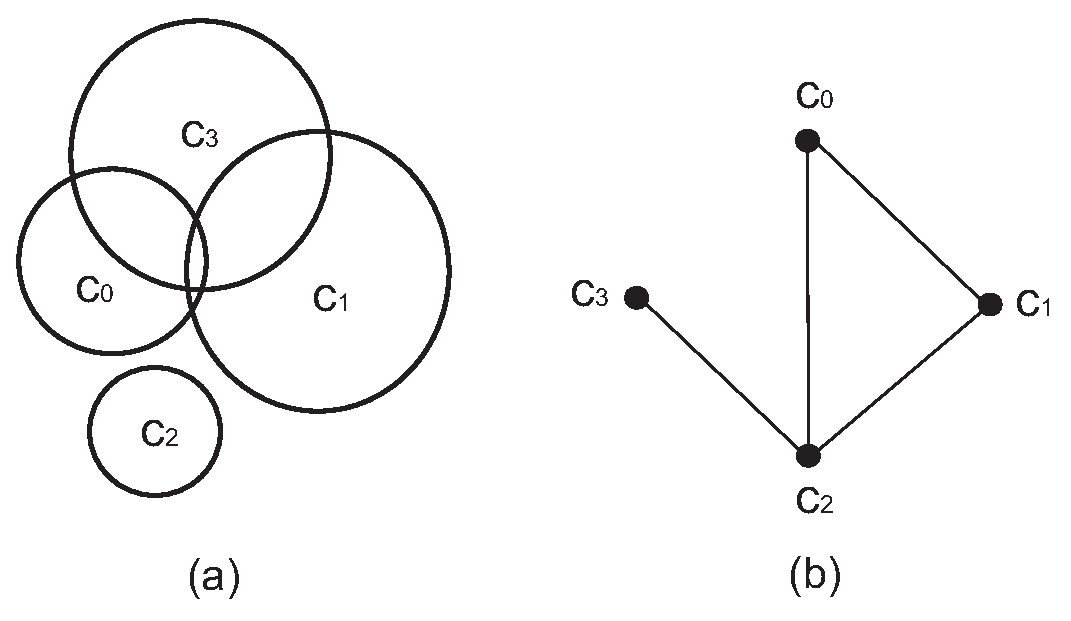
\epsfig{file=figure/graph_model.eps,width=0.8\columnwidth}
\caption{(a) 4 concepts in the entity space
(b) corresponding concept graph
}
\label{fig:graph_model}
\end{figure}

The argument conceptualization problem is then transformed to
finding the $k$-clique with maximum combined weight.

A straightforward way to define the weight for each concept is
counting the number of argument instances it subsumes according to the
IsA taxonomy. This assumes that all argument instances of a verb are of
equal importance, which is not true in general.
We thus generalize the importance of an argument $e$ to a verb $v$
by a quality function $Q_v(e)$, which we will discuss in detail
in \secref{sec:qe}.
Consequently, the weight of concept $c$ for verb $v$ is
defined as
\begin{equation}
w_v(c)=\sum_{e\in \{e|e\;\text{isA}\;c\}}{Q_v(e)}
\end{equation}
The argument conceptualization problem is to find
a $k$-clique (which forms a concept set as $C_k$)
in the graph $G$ which maximizes
\begin{equation}
\label{eq:f}
f_v(C_k)=\sum_{c\in C_k}{w_v(c)}.
\end{equation}

The reason for parameterizing the number of argument concepts of a
verb is i) different verbs have different number of senses; and ii)
even for the same verb, there's no agreement on the exact number of its
senses because one meaning can always be divided into a number of
finer-grain meanings, depending on how you view the semantics.
For example, in Oxford English Dictionary~\cite{oxford},
the transitive verb ``eat'' has 4 senses (or definitions),
while in Cambridge Dictionary~\cite{cambridge} it has just one meaning.
Thus in this paper, we choose
to model the number of argument concepts as an input of the problem.
